% Compile from this directory with: pdflatex binary-search-tree.tex
\documentclass[tikz,border=1pt]{standalone}
\usepackage[T1]{fontenc}
\usepackage{helvet}
\usetikzlibrary{arrows.meta}

\begin{document}
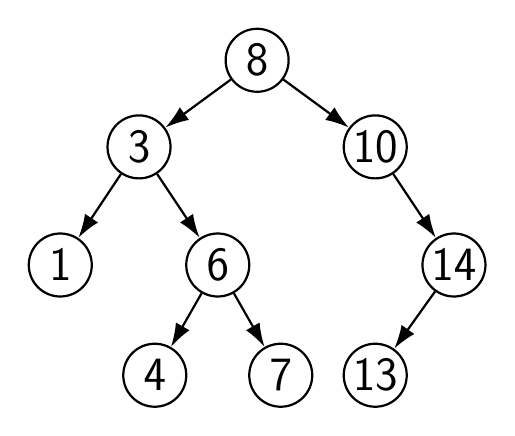
\begin{tikzpicture}[
    vertex/.style={
        circle, draw, line width=0.8pt,
        minimum size=8mm, inner sep=0pt,
        font=\sffamily\fontsize{18}{18}\selectfont
    },
    edge/.style={line width=0.8pt, -{Latex[length=3mm,width=2mm]}}
]
    % Explicit positions preserve the layout of the original illustration.
    \node[vertex] (n8)  at ( 0.0, 0.0) {8};
    \node[vertex] (n3)  at (-1.5,-1.1) {3};
    \node[vertex] (n10) at ( 1.5,-1.1) {10};
    \node[vertex] (n1)  at (-2.5,-2.6) {1};
    \node[vertex] (n6)  at (-0.5,-2.6) {6};
    \node[vertex] (n14) at ( 2.5,-2.6) {14};
    \node[vertex] (n4)  at (-1.3,-4.0) {4};
    \node[vertex] (n7)  at ( 0.3,-4.0) {7};
    \node[vertex] (n13) at ( 1.5,-4.0) {13};

    \foreach \parent/\child in {8/3,8/10,3/1,3/6,6/4,6/7,10/14,14/13}
        \draw[edge] (n\parent) -- (n\child);
\end{tikzpicture}
\end{document}
